\providecommand{\qcOne}{\mathbf{1}}   %
\providecommand{\qcTwo}{\mathbf{2}}   %
\providecommand{\qcor}[1]{\ulcorner#1\urcorner}   %
\providecommand{\Cat}{\mathcal{C}at}
\providecommand{\QCat}{\mathcal{Q}\mathcal{C}at}

\section{纤维化伴随与纤维化等价}\label{sec:fibered-adjunctions-and-fibered-equivalences}

在命题 3.2.10 中，我们发现 $A$ 中的箭头\trInfinityCategory{} $A^{2}$ 连同其余定义域与%
定义域求值函子 $(p_{1},p_{0})\colon A^{2}\to A\times A$ 在\trHomotopyTwoCategory{}中满足一个%
弱\trUniversalProperty，把它在 $A\times A$ 之上刻划直至\trEquivalence。类似地，命题 3.4.11 告诉%
我们：与一对具有公共余定义域的\trFunctor{}相配的\trCommaInfinityCategory{}被刻划直至%
\trFiberedEquivalence{}（如定义 3.2.7 中所定义）。

如警告 3.2.9 中所述，关于指定一个\trFiberedEquivalence{}所需的 2-范畴数据尚有几分含糊，我们%
现在正面处理这一问题。问题在于：对\trInfinityCosmos{} $\mathcal{K}$ 中的一个\trInfinityCategory{} %
$B$，切片\trInfinityCosmos{}的\trHomotopyTwoCategory{} $\mathbb{h}(\mathcal{K}_{/B})$（见命题 1.2.22 与%
定义 1.4.1）并不同构于 2-范畴 $(\mathbb{h}\mathcal{K})_{/B}$——即 $\mathbb{h}\mathcal{K}$ 中居于 %
$B$ 之上的\trIsofibration、\trFunctor{}与 2-\trCell{}构成的 2-范畴。然而，有一个联系这两个 2-范畴的%
典范比较函子，它满足一个我们现在引入的性质：

\begin{definition}[覆盖 2-函子]\label{def:smothering-two-functor}
2-\trTwoFunctor{} $F\colon\mathcal{A}\to\mathcal{B}$ 称为\trSmothering，若它：
\begin{itemize}
\item 在对象上满射；
\item 在 1-\trCell{}上满：对 $\mathcal{A}$ 中任何一对对象 $A,A'$ 与 $\mathcal{B}$ 中的任何 %
1-\trCell{} $k\colon FA\to FA'$，存在 $\mathcal{A}$ 中的 $f\colon A\to A'$ 使得 $Ff=k$；
\item 在 2-\trCell{}上满：对 $\mathcal{A}$ 中任何平行 1-\trCell{}对 $f,g\colon A\to A'$ 与 %
$\mathcal{B}$ 中形如 $FA\underset{\scriptstyle Fg}{\overset{\scriptstyle Ff}{\Rightarrow}}FA'$ %
的 2-\trCell{} $\beta\colon Ff\Rightarrow Fg$，存在 $\mathcal{A}$ 中的 2-\trCell{} %
$\alpha\colon f\Rightarrow g$ 使得 $F\alpha=\beta$；以及
\item 在 2-\trCell{}上保守：对 $\mathcal{A}$ 中的任何 2-\trCell{} $\alpha$，若 $F\alpha$ 在 %
$\mathcal{B}$ 中\trInvertible，则 $\alpha$ 在 $\mathcal{A}$ 中\trInvertible。
\end{itemize}
\end{definition}

这即是说，覆盖 2-函子是一个在对象上满射的 2-\trTwoFunctor，它是「局部\trSmothering」的——%
意即其在\trHomCategory{}上的作用经由一个\trSmotheringFunctor{}进行，如定义 3.1.2 所编定。
覆盖 2-函子的原型例子解出练习 1.4.vii。

\begin{proposition}\label{prop:canonical-comparison}
设 $B$ 是\trInfinityCosmos{} $\mathcal{K}$ 中的一个\trInfinityCategory。存在一个典范 %
2-\trTwoFunctor
\[
\mathbb{h}(\mathcal{K}_{/B})\longrightarrow(\mathbb{h}\mathcal{K})_{/B}
\]
从切片\trInfinityCosmos{} $\mathcal{K}_{/B}$ 的\trHomotopyTwoCategory{}指向「$\mathbb{h}\mathcal{K}$ %
中居于 $B$ 之上的\trIsofibration、\trFunctor{}与 2-\trCell{}」的 2-范畴，且此 2-\trTwoFunctor{}是%
\trSmothering。
\end{proposition}

这或多或少立刻可以从引理 3.1.5 得出，但我们仍把细节一一写出。

\begin{proof}
2-范畴 $\mathbb{h}(\mathcal{K}_{/B})$ 与 $(\mathbb{h}\mathcal{K})_{/B}$ 具有相同的对象——%
余定义域为 $B$ 的\trIsofibration——与相同的 1-\trCell——诸定义域之间同这些\trIsofibration{}相交换的%
\trFunctor——故可把典范映射定义为在底 1-范畴上取恒同。

据命题 1.2.22 给出的切片\trInfinityCosmos{}之定义，从 $p\colon E\twoheadrightarrow B$ 到 %
$q\colon F\twoheadrightarrow B$ 的诸\trFunctor{} $f,g\colon E\to F$ 之间的一个 2-\trCell{}是下左单纯集 %
\trPullback{}所定义的\trQuasiCategory{}中 1-\trSimplex{}的一个\trHomotopy{}类
\begin{center}
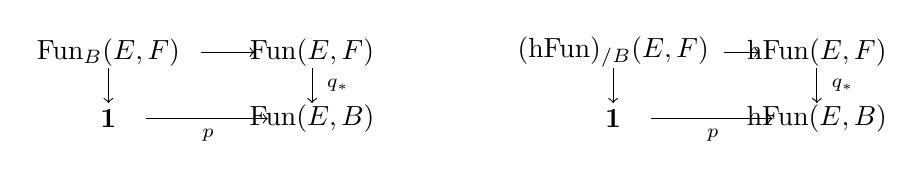
\begin{tikzpicture}[x=1.6em,y=1.6em]
  \node (tl) at (0,1.5) {$\mathrm{Fun}_{B}(E,F)$};
  \node (tr) at (4.6,1.5) {$\mathrm{Fun}(E,F)$};
  \node (bl) at (0,0) {$\qcOne$};
  \node (br) at (4.6,0) {$\mathrm{Fun}(E,B)$};
  \draw[->] (2.1,1.5) -- (3.3,1.5);
  \node at (0.52,1.02) {$\scriptstyle\lrcorner$};
  \draw[->] (0,1.15) -- (0,0.35);
  \draw[->] (4.6,1.15) -- (4.6,0.35);
  \node at (5.18,0.75) {$\scriptstyle q_{*}$};
  \draw[->] (0.85,0) -- (3.6,0);
  \node at (2.25,-0.38) {$\scriptstyle p$};
  \begin{scope}[shift={(11.4,0)}]
  \node (tl2) at (0,1.5) {$(\mathrm{hFun})_{/B}(E,F)$};
  \node (tr2) at (4.6,1.5) {$\mathrm{hFun}(E,F)$};
  \node (bl2) at (0,0) {$\qcOne$};
  \node (br2) at (4.6,0) {$\mathrm{hFun}(E,B)$};
  \draw[->] (2.5,1.5) -- (3.3,1.5);
  \node at (0.52,1.02) {$\scriptstyle\lrcorner$};
  \draw[->] (0,1.15) -- (0,0.35);
  \draw[->] (4.6,1.15) -- (4.6,0.35);
  \node at (5.18,0.75) {$\scriptstyle q_{*}$};
  \draw[->] (0.85,0) -- (3.6,0);
  \node at (2.25,-0.38) {$\scriptstyle p$};
  \end{scope}
\end{tikzpicture}
\end{center}
展开来说，一个 2-\trCell{} $\alpha\colon f\Rightarrow g$ 由 $\mathrm{Fun}(E,F)$ 中的一条 %
1-\trSimplex{} $\alpha\colon f\to g$ 所表示，后者与 $q$ 作\trWhiskering{}后给出顶点 %
$p\in\mathrm{Fun}(E,B)$ 上的退化 1-\trSimplex；两条这样的 1-\trSimplex{}表示同一个 2-\trCell，%
当且仅当它们围成一个形如 (1.1.8) 中所示形状的 2-\trSimplex，且后者与 $q$ 作\trWhiskering{}后给出 %
$p$ 上的退化 2-\trSimplex。

相比之下，$(\mathbb{h}\mathcal{K})_{/B}$ 中的一个 2-\trCell{}是上右范畴\trPullback{}所定义的范畴中的%
一个态射。这样的 2-\trCell{}由 $\mathrm{Fun}(E,F)$ 中的 1-\trSimplex{} $\alpha\colon f\to g$ 表示，%
后者与 $q$ 作\trWhiskering{}后给出 $\mathrm{Fun}(E,B)$ 中与 $p$ 上的退化 1-\trSimplex{}
\trHomotopic{}1-\trSimplex；两条这样的 1-\trSimplex{}表示同一个 2-\trCell，当且仅当它们在 %
$\mathrm{Fun}(E,F)$ 中\trHomotopic。

把\trHomotopyCategory{}函子 $\mathrm{h}\colon\QCat\to\Cat$ 应用于上左\trPullback，得到张在上右%
\trPullback{}之上的一个\trCone，从而诱导典范映射
\[
\mathrm{h}(\mathrm{Fun}_{B}(E,F))\longrightarrow(\mathrm{hFun})_{/B}(E,F),
\]
它正是典范 2-\trTwoFunctor{} $\mathbb{h}(\mathcal{K}_{/B})\to(\mathbb{h}\mathcal{K})_{/B}$ 在 %
\trHomCategory{}上的作用。由引理 3.1.5，这个典范映射定义一个在对象上双射的\trSmotheringFunctor。%
于是，我们定义了一个 2-\trTwoFunctor{} $\mathbb{h}(\mathcal{K}_{/B})\to(\mathbb{h}\mathcal{K})_{/B}$，%
它在 0-与 1-\trCell{}上双射且局部\trSmothering，如所宣称。
\end{proof}

严格说来，覆盖 2-函子并不可逆，但余定义域处的 2-范畴结构依然能够提升到定义域。

\begin{lemma}\label{lem:smothering-reflect-create}
覆盖 2-函子反射并创造\trEquivalence。
\end{lemma}

\begin{proof}
对任何覆盖 2-函子 $F\colon\mathcal{A}\to\mathcal{B}$ 与 $\mathcal{A}$ 中的 1-\trCell{} %
$f\colon A\to B$，若 $Ff\colon FA\simeq FB$ 是 $\mathcal{B}$ 中的一个\trEquivalence，则由 %
1-\trCell{}上的满性，$Ff$ 的一个等价逆 $g'\colon FB\simeq FA$ 提升为 $\mathcal{A}$ 中的 %
1-\trCell{} $g\colon B\to A$。由 2-\trCell{}上的满性，\trIsomorphism{} %
$\mathrm{id}_{FA}\cong g'\circ Ff$ 与 $Ff\circ g'\cong\mathrm{id}_{FB}$ 也提升到 $\mathcal{A}$，%
而由 2-\trCell{}上的保守性，这些提升后的 2-\trCell{}也\trInvertible。这证明\trEquivalence{}被反射。%
为见它们被创造，注意 $\mathcal{B}$ 中的任何 $f'\colon FA\simeq FB$ 都提升为 1-\trCell{} %
$f\colon A\to B$，由刚才给出的构造它是一个\trEquivalence。
\end{proof}

将\cref{lem:smothering-reflect-create}应用于覆盖 2-函子
\[
\mathbb{h}(\mathcal{K}_{/B})\longrightarrow(\mathbb{h}\mathcal{K})_{/B}
\]
我们便一举解决了关于\trFiberedEquivalence{}之 2-范畴数据的含糊性。

\begin{proposition}[纤维化等价数据]\label{prop:fibered-equivalence-data}
设 $B$ 是\trInfinityCosmos{} $\mathcal{K}$ 中的一个\trInfinityCategory。
\begin{enumerate}[label=(\roman*)]
\item $(\mathbb{h}\mathcal{K})_{/B}$ 中的任何\trEquivalence{}都提升为 $\mathbb{h}(\mathcal{K}_{/B})$ %
中的\trEquivalence。也就是说，$B$ 之上的\trFiberedEquivalence{}可以这样给定：指定 $B$ 之上的%
一对对立 1-\trCell{} $f\colon E\to F$ 与 $g\colon F\to E$，连同居于 $\mathbb{h}\mathcal{K}$ 中 %
$B$ 之上的可逆 2-\trCell{} $\mathrm{id}_{E}\cong gf$ 与 $fg\cong\mathrm{id}_{F}$。
\item 此外，若 $f\colon E\to F$ 是 $B$ 上的诸\trIsofibration{}之间的一个映射，且它容许一个未必 %
纤维化的等价逆 $g\colon F\to E$、连同未必纤维化的 2-\trCell{} $\mathrm{id}_{E}\cong gf$ 与 %
$fg\cong\mathrm{id}_{F}$，则这些数据\trIsomorphism{}于一个真正的\trFiberedEquivalence。
\end{enumerate}
于是，遗忘 2-函子 $\mathbb{h}(\mathcal{K}_{/B})\to(\mathbb{h}\mathcal{K})_{/B}\to\mathbb{h}\mathcal{K}$ %
反射\trEquivalence。
\end{proposition}

\begin{proof}
第一款由\cref{lem:smothering-reflect-create}与\cref{prop:canonical-comparison}得证。第二款断言 %
遗忘 2-函子 $(\mathbb{h}\mathcal{K})_{/B}\to\mathbb{h}\mathcal{K}$ 反射\trEquivalence，留作 %
\cref{ex:ambient-equivalence}，它只需要\trIsofibration{}的 2-范畴提升性质（见命题 1.4.9）。
\end{proof}
这给出命题 1.2.22(vii) 的一个 2-范畴论证明：对\trInfinityCosmos{} $\mathcal{K}$ 中的任何%
\trInfinityCategory{} $B$，\trForgetfulFunctor{} $\mathcal{K}_{/B}\to\mathcal{K}$ 保持并反射%
\trEquivalence。覆盖 2-函子 $\mathbb{h}(\mathcal{K}_{/B})\to(\mathbb{h}\mathcal{K})_{/B}$ 也可以用来把那些在 %
$B$ 之上 2-范畴式纤维化的\trAdjunction{}提升为切片\trInfinityCosmos{} $\mathcal{K}_{/B}$ 中的 %
\trAdjunction。

\begin{definition}[\trFiberedAdjunction]\label{def:fibered-adjunction}
\trInfinityCosmos{} $\mathcal{K}$ 中\trInfinityCategory{} $B$ 之上的一个\textbf{\trFiberedAdjunction}%
（fibered adjunction）是切片\trInfinityCosmos{} $\mathcal{K}_{/B}$ 中的一个\trAdjunction。
\begin{center}
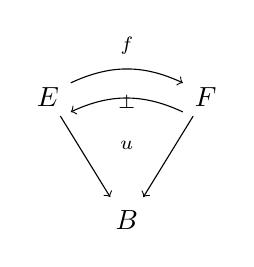
\begin{tikzpicture}[x=1.5em,y=1.5em]
  \node (e) at (-1.9,1.2) {$E$};
  \node (f) at (1.9,1.2) {$F$};
  \draw[->] (-1.35,1.55) to[bend left=25] (1.35,1.55);
  \node at (0,2.45) {$\scriptstyle f$};
  \node at (0,1.1) {$\scriptstyle\perp$};
  \draw[->] (1.35,0.85) to[bend right=25] (-1.35,0.85);
  \node at (0,0.05) {$\scriptstyle u$};
  \draw[->] (-1.6,0.75) -- (-0.4,-1.2);
  \draw[->] (1.6,0.75) -- (0.4,-1.2);
  \node (b) at (0,-1.75) {$B$};
\end{tikzpicture}
\end{center}
\end{definition}

我们写 $f\dashv_{B}u$，以指示 $B$ 之上的给定诸\trFunctor{}是\textbf{在 $B$ 上伴随}（adjoint over %
$B$）的。

\begin{lemma}[\trFiberedAdjunction{}的拉回与投影]\label{lem:fibered-adjunction-pullback-projection}
\begin{enumerate}[label=(\roman*)]
\item $B$ 之上的一个\trFiberedAdjunction{}沿任何\trFunctor{} $k\colon A\to B$ 拉回，定义 $A$ 之上的一个 %
\trFiberedAdjunction。
\item $A$ 之上的一个\trFiberedAdjunction{}可以与任何\trIsofibration\footnote{我们要求 $p$ 是一个 %
\trIsofibration，这是缘于我们的约定：切片\trInfinityCosmos{}中的对象是固定底之上的%
\trIsofibration。} $p\colon A\twoheadrightarrow B$ 复合，定义 $B$ 之上的一个\trFiberedAdjunction。
\end{enumerate}
\end{lemma}

\begin{proof}
对任何\trInfinityCosmos{} $\mathcal{K}$，沿 $k\colon A\to B$ 取\trPullback{}定义一个%
\trCosmologicalFunctor{} $k^{*}\colon\mathcal{K}_{/B}\to\mathcal{K}_{/A}$（据命题 1.3.4(v)），%
它下降为一个 2-\trTwoFunctor{} $k^{*}\colon\mathbb{h}(\mathcal{K}_{/B})\to\mathbb{h}(\mathcal{K}_{/A})$，%
把 $B$ 之上的\trFiberedAdjunction{}带到 $A$ 之上的\trFiberedAdjunction。这证明 (i)。

与一个\trIsofibration{} $p\colon A\twoheadrightarrow B$ 复合也定义诸切片的一个 2-\trTwoFunctor{} %
$p_{*}\colon\mathbb{h}(\mathcal{K}_{/A})\to\mathbb{h}(\mathcal{K}_{/B})$。于是，与一个 %
\trIsofibration{}复合把 $A$ 之上的\trFiberedAdjunction{}带到 $B$ 之上的\trFiberedAdjunction，证得 (ii)。
\end{proof}

与\cref{lem:smothering-reflect-create}相类比：

\begin{lemma}\label{lem:smothering-lift-adjunctions}
若 $F\colon\mathcal{A}\to\mathcal{B}$ 是一个覆盖 2-函子，则 $\mathcal{B}$ 中的任何\trAdjunction{}%
都可提升为 $\mathcal{A}$ 中的\trAdjunction。特别地，\trInfinityCosmos{} $\mathcal{K}$ 的切片 %
2-范畴 $(\mathbb{h}\mathcal{K})_{/B}$ 中的任何\trAdjunction{}都提升为 $B$ 之上的一个\trFiberedAdjunction。
\end{lemma}

\begin{proof}
\cref{ex:smothering-lifts-adjunctions}。
\end{proof}

组合\cref{def:fibered-adjunction}与定义 2.2.1，我们得到纤维化始元素与纤维化终元素的概念。

\begin{definition}\label{def:fibered-initial-terminal-element}
给定一个\trIsofibration{} $p\colon E\twoheadrightarrow B$，我们说 $E$ \textbf{容许 $B$ 上的一个 %
始元素}（initial element over $B$）或\textbf{容许 $B$ 上的一个终元素}（terminal element over %
$B$），若对 $B$ 之上从 $p$ 到 $\mathrm{id}_{B}$ 的唯一\trFunctor，分别存在一个纤维化%
\trLeftAdjoint{}或纤维化\trRightAdjoint：
\begin{center}
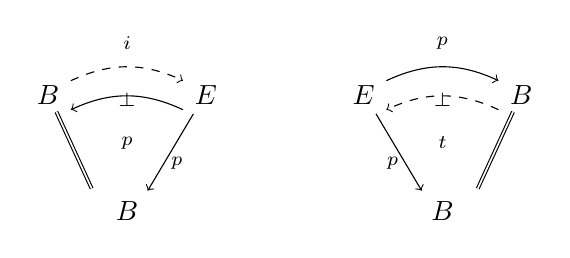
\begin{tikzpicture}[x=1.5em,y=1.5em]
  \node (bl) at (-1.9,1.2) {$B$};
  \node (er) at (1.9,1.2) {$E$};
  \draw[->,dashed] (-1.35,1.55) to[bend left=25] (1.35,1.55);
  \node at (0,2.45) {$\scriptstyle i$};
  \node at (0,1.1) {$\scriptstyle\perp$};
  \draw[->] (1.35,0.85) to[bend right=25] (-1.35,0.85);
  \node at (0,0.05) {$\scriptstyle p$};
  \draw[double] (-1.7,0.8) -- (-0.85,-1.05);
  \draw[->] (1.6,0.75) -- (0.5,-1.1);
  \node at (1.2,-0.45) {$\scriptstyle p$};
  \node (bb) at (0,-1.6) {$B$};
  \begin{scope}[shift={(7.6,0)}]
  \node (el) at (-1.9,1.2) {$E$};
  \node (br) at (1.9,1.2) {$B$};
  \draw[->] (-1.35,1.55) to[bend left=25] (1.35,1.55);
  \node at (0,2.45) {$\scriptstyle p$};
  \node at (0,1.1) {$\scriptstyle\perp$};
  \draw[->,dashed] (1.35,0.85) to[bend right=25] (-1.35,0.85);
  \node at (0,0.05) {$\scriptstyle t$};
  \draw[double] (1.7,0.8) -- (0.85,-1.05);
  \draw[->] (-1.6,0.75) -- (-0.5,-1.1);
  \node at (-1.2,-0.45) {$\scriptstyle p$};
  \node (bb2) at (0,-1.6) {$B$};
  \end{scope}
\end{tikzpicture}
\end{center}
\end{definition}

也就是说，$E$ 容许 $B$ 上的始元素或终元素，恰好当把 $p\colon E\twoheadrightarrow B$ 视为 %
$B$ 之上的切片\trInfinityCosmos{}的一个对象时，$p$ 容许始元素或终元素。

下一条结果表明：纤维化始元素或纤维化终元素存在，恰好当\trIsofibration{} $p\colon E\to B$ 分别 %
容许一个\textbf{\trLeftAdjoint\trRightInverse}（left adjoint right inverse）或%
\trRightAdjoint\trRightInverse{}时。

\begin{lemma}\label{lem:rajri-fibered-adjunction}
设 $p\colon E\twoheadrightarrow B$ 是任何容许\trRightAdjoint\trRightInverse{} $r'\colon B\to E$ %
的\trIsofibration。则 $r'$ \trIsomorphism{}于一个定义\trFiberedAdjunction{}的\trFunctor{} $r$：
\begin{center}
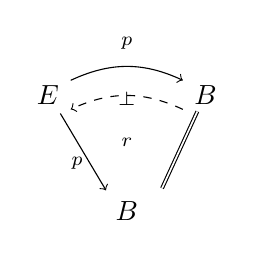
\begin{tikzpicture}[x=1.5em,y=1.5em]
  \node (el) at (-1.9,1.2) {$E$};
  \node (br) at (1.9,1.2) {$B$};
  \draw[->] (-1.35,1.55) to[bend left=25] (1.35,1.55);
  \node at (0,2.45) {$\scriptstyle p$};
  \node at (0,1.1) {$\scriptstyle\perp$};
  \draw[->,dashed] (1.35,0.85) to[bend right=25] (-1.35,0.85);
  \node at (0,0.05) {$\scriptstyle r$};
  \draw[double] (1.7,0.8) -- (0.85,-1.05);
  \draw[->] (-1.6,0.75) -- (-0.5,-1.1);
  \node at (-1.2,-0.45) {$\scriptstyle p$};
  \node (bb) at (0,-1.6) {$B$};
\end{tikzpicture}
\end{center}
于是，一个\trIsofibration{} $p\colon E\twoheadrightarrow B$ 容许%
\trRightAdjoint\trRightInverse，当且仅当 $E$ 容许 $B$ 上的一个终元素。
\end{lemma}

\begin{proof}
由于\trInfinityCosmos{} $\mathcal{K}$ 中的一个\trIsofibration{} $p\colon E\twoheadrightarrow B$ 在 %
\trHomotopyTwoCategory{} $\mathbb{h}\mathcal{K}$ 中定义一个\trIsofibration，\trAdjunction{} %
$p\dashv r'$ 的可逆\trCounit{} $\epsilon'\colon pr'\cong\mathrm{id}_{B}$ 提升为定义一个\trFunctor{} %
$r\colon B\to E$ 连同一个自然\trIsomorphism{} $\gamma\colon r'\cong r$，使得 $p\gamma=\epsilon'$ %
且 $pr=\mathrm{id}_{B}$：
\begin{center}
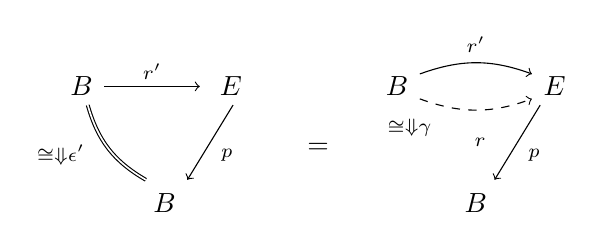
\begin{tikzpicture}[x=1.5em,y=1.5em]
  \node (b1) at (-2.1,1.2) {$B$};
  \node (e1) at (1.5,1.2) {$E$};
  \draw[->] (-1.55,1.2) -- (0.75,1.2);
  \node at (-0.4,1.56) {$\scriptstyle r'$};
  \draw[double] (-1.95,0.75) to[bend right=22] (-0.55,-1.05);
  \node at (-2.6,-0.45) {$\scriptstyle\cong\Downarrow\epsilon'$};
  \draw[->] (1.55,0.75) -- (0.45,-1.05);
  \node at (1.4,-0.45) {$\scriptstyle p$};
  \node (bb1) at (-0.1,-1.6) {$B$};
  \node at (3.6,-0.3) {$=$};
  \begin{scope}[shift={(7.4,0)}]
  \node (b2) at (-1.9,1.2) {$B$};
  \node (e2) at (1.9,1.2) {$E$};
  \draw[->] (-1.35,1.5) to[bend left=20] (1.35,1.5);
  \node at (0,2.2) {$\scriptstyle r'$};
  \draw[->,dashed] (-1.35,0.9) to[bend right=20] (1.35,0.9);
  \node at (-1.6,0.2) {$\scriptstyle\cong\Downarrow\gamma$};
  \node at (0.1,-0.15) {$\scriptstyle r$};
  \draw[->] (1.55,0.75) -- (0.45,-1.05);
  \node at (1.4,-0.45) {$\scriptstyle p$};
  \node (bb2) at (0,-1.6) {$B$};
  \end{scope}
\end{tikzpicture}
\end{center}
据练习 2.1.ii 中留给读者的构造，$p\dashv r$ 带有\trUnit{} $\eta:=\gamma p\cdot\eta'$——由原先的%
\trUnit{} $\eta'$ 与 $\gamma$ 复合而定义——以及\trCounit{} $\epsilon:=\epsilon'\cdot p\gamma^{-1}$。%
特别地，由于 $p\gamma=\epsilon'$，\trCounit{} $\epsilon$ 是恒同 2-\trCell，从而诸\trTriangleEqualities{}%
复合之一约化为断言 $p\eta=\mathrm{id}_{p}$。
\end{proof}

这构造了 $p$——视为 $(\mathbb{h}\mathcal{K})_{/B}$ 中的一个\trFunctor——的一个\trRightAdjoint。由 %
\cref{lem:smothering-lift-adjunctions}，这个伴随沿\cref{prop:canonical-comparison}的覆盖 2-函子提升，%
定义 $\mathbb{h}(\mathcal{K}_{/B})$ 中所需要形状的 $B$ 之上\trFiberedAdjunction（见 %
\cref{ex:smothering-lifts-adjunctions}）。\cref{def:fibered-initial-terminal-element}把刚构造的 %
\trFiberedAdjunction{}解释为 $E$ 中 $B$ 上的一个终元素。

有了这一观察，定理 3.5.12 可以更紧凑地总结如下：

\begin{corollary}\label{cor:right-representability-terminal-element}
对任何\trCospan{} $C\xrightarrow{\;g\;}A\xleftarrow{\;f\;}B$，\trCommaInfinityCategory{} %
$\mathrm{Hom}_{A}(f,g)$ 是右可表示的，当且仅当 $\mathrm{Hom}_{A}(f,g)$ 容许 $C$ 上的一个终元素——%
此时表示\trFunctor{}定义 $g$ 穿过 $f$ 的一个绝对右提升。
\end{corollary}

\begin{remark}\label{rem:analytic-synthetic}
在一个由 $(\infty,1)$-范畴构成的\trInfinityCosmos{}中，可表示性定理还可以进一步改进为：%
$\mathrm{Hom}_{A}(f,g)$ 是右可表示的，当且仅当对所有\trElement{} $c\colon\qcOne\to C$，%
∞-范畴 $\mathrm{Hom}_{A}(f,gc)$ 具有一个终元素（见推论 12.2.8）。该证明需要「解析的」技术，%
与本章中纯粹「合成的」推理形成对照。
\end{remark}

\begin{example}\label{exa:terminal-element-hom}
由引理 3.5.9 与\cref{lem:rajri-fibered-adjunction}，对任何\trFunctor{} $f\colon A\to B$，存在 %
\trFiberedAdjunction
\begin{center}
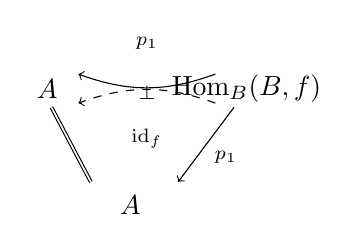
\begin{tikzpicture}[x=1.5em,y=1.5em]
  \node (a) at (-2.4,1.2) {$A$};
  \node (h) at (2.4,1.2) {$\mathrm{Hom}_{B}(B,f)$};
  \draw[->] (1.65,1.55) to[bend left=20] (-1.65,1.55);
  \node at (0,2.3) {$\scriptstyle p_{1}$};
  \node at (0,1.1) {$\scriptstyle\perp$};
  \draw[->,dashed] (1.65,0.85) to[bend right=20] (-1.65,0.85);
  \node at (0,0.0) {$\scriptstyle\qcor{\mathrm{id}_{f}}$};
  \draw[double] (-2.3,0.75) -- (-1.35,-1.05);
  \draw[->] (2.1,0.75) -- (0.75,-1.05);
  \node at (1.9,-0.45) {$\scriptstyle p_{1}$};
  \node (ab) at (-0.4,-1.6) {$A$};
\end{tikzpicture}
\end{center}
它断言 $\qcor{\mathrm{id}_{f}}\colon A\to\mathrm{Hom}_{B}(B,f)$ 定义 $\mathrm{Hom}_{B}(B,f)$ 中 %
$A$ 上的一个终元素。

由\cref{lem:fibered-adjunction-pullback-projection}(i)，可以把这个\trFiberedAdjunction{}沿任何\trElement{} %
$a\colon\qcOne\to A$ 拉回，得到一个\trAdjunction，它甄别出纤维
\begin{center}
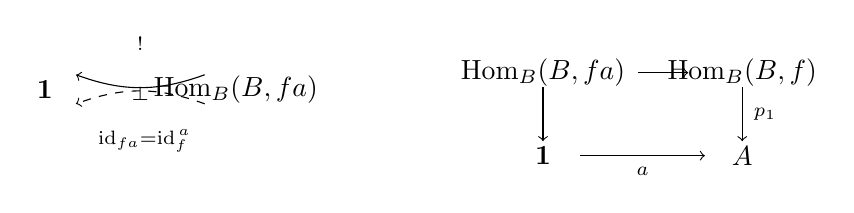
\begin{tikzpicture}[x=1.5em,y=1.5em]
  \node (one) at (-2.4,1.2) {$\qcOne$};
  \node (hfa) at (2.2,1.2) {$\mathrm{Hom}_{B}(B,fa)$};
  \draw[->] (1.45,1.55) to[bend left=20] (-1.65,1.55);
  \node at (-0.1,2.3) {$\scriptstyle !$};
  \node at (-0.1,1.1) {$\scriptstyle\perp$};
  \draw[->,dashed] (1.45,0.85) to[bend right=20] (-1.65,0.85);
  \node at (0,-0.05) {$\scriptstyle\qcor{\mathrm{id}_{fa}}=\qcor{\mathrm{id}_{f}}^{\,a}$};
  \begin{scope}[shift={(9.6,0)}]
  \node (hfa2) at (0,1.6) {$\mathrm{Hom}_{B}(B,fa)$};
  \node (hf) at (4.8,1.6) {$\mathrm{Hom}_{B}(B,f)$};
  \node (o2) at (0,-0.4) {$\qcOne$};
  \node (a2) at (4.8,-0.4) {$A$};
  \draw[->] (2.3,1.6) -- (3.5,1.6);
  \node at (0.52,1.12) {$\scriptstyle\lrcorner$};
  \draw[->] (0,1.25) -- (0,-0.05);
  \draw[->] (4.8,1.25) -- (4.8,-0.05);
  \node at (5.35,0.6) {$\scriptstyle p_{1}$};
  \draw[->] (0.9,-0.4) -- (3.9,-0.4);
  \node at (2.4,-0.78) {$\scriptstyle a$};
  \end{scope}
\end{tikzpicture}
\end{center}
中的一个终元素，推广了推论 3.5.10 的结果。
\end{example}

\begin{example}[复合的\trFiberedAdjunction]\label{exa:fibered-adjoints-composition}
对任何\trInfinityCategory{} $A$，引理 2.1.14 中构造的「复合」函子 %
$\circ\colon A^{2}\times_{A}A^{2}\to A^{2}$ 的诸伴随，由复合一个伴随\trFunctor{}三元组而构造，%
此三元组纤维化于\trEndpointEvaluation{}函子之上
\begin{center}
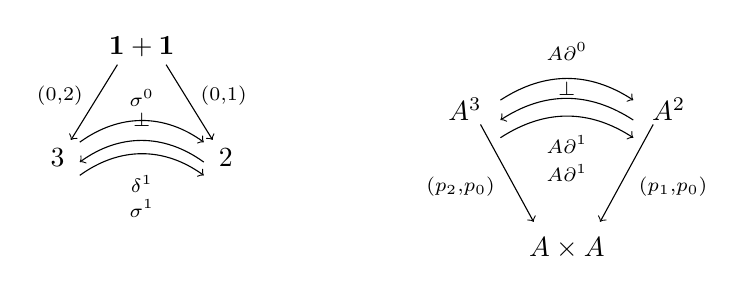
\begin{tikzpicture}[x=1.6em,y=1.6em]
  \node (sum) at (0,2.7) {$\qcOne+\qcOne$};
  \node (three) at (-1.9,0.2) {$3$};
  \node (two) at (1.9,0.2) {$2$};
  \draw[->] (-0.55,2.3) -- (-1.6,0.6);
  \node at (-1.85,1.6) {$\scriptstyle(0,2)$};
  \draw[->] (0.55,2.3) -- (1.6,0.6);
  \node at (1.85,1.6) {$\scriptstyle(0,1)$};
  \draw[->] (-1.4,0.55) .. controls (-0.5,1.2) and (0.5,1.2) .. (1.4,0.55);
  \node at (0,1.55) {$\scriptstyle\sigma^{0}$};
  \node at (0,1.05) {$\scriptstyle\perp$};
  \draw[->] (1.4,0.1) .. controls (0.5,0.75) and (-0.5,0.75) .. (-1.4,0.1);
  \node at (0,-0.4) {$\scriptstyle\delta^{1}$};
  \draw[->] (-1.4,-0.2) .. controls (-0.5,0.45) and (0.5,0.45) .. (1.4,-0.2);
  \node at (0,-0.95) {$\scriptstyle\sigma^{1}$};
  \node at (4.8,0.9) {$\rightsquigarrow$};
  \begin{scope}[shift={(9.6,0)}]
  \node (a3) at (-2.3,1.3) {$A^{3}$};
  \node (a2) at (2.3,1.3) {$A^{2}$};
  \draw[->] (-1.5,1.5) .. controls (-0.5,2.15) and (0.5,2.15) .. (1.5,1.5);
  \node at (0,2.6) {$\scriptstyle A\partial^{0}$};
  \node at (0,1.75) {$\scriptstyle\perp$};
  \draw[->] (1.5,1.05) .. controls (0.5,1.7) and (-0.5,1.7) .. (-1.5,1.05);
  \node at (0,0.5) {$\scriptstyle A\partial^{1}$};
  \draw[->] (-1.5,0.65) .. controls (-0.5,1.3) and (0.5,1.3) .. (1.5,0.65);
  \node at (0,-0.15) {$\scriptstyle A\partial^{1}$};
  \draw[->] (-1.95,0.95) -- (-0.75,-1.25);
  \node at (-2.4,-0.45) {$\scriptstyle(p_{2},p_{0})$};
  \draw[->] (1.95,0.95) -- (0.75,-1.25);
  \node at (2.4,-0.45) {$\scriptstyle(p_{1},p_{0})$};
  \node (axa) at (0,-1.85) {$A\times A$};
  \end{scope}
\end{tikzpicture}
\end{center}
连同涉及\trFunctor{} $A^{3}\rightleftarrows A^{2}\times_{A}A^{2}$ 的一个伴随等价——后者同样居于 %
$A\times A$ 之上。\cref{lem:rajri-fibered-adjunction}及其对偶蕴含：这些伴随等价可以提升为 %
$A\times A$ 之上的\trFiberedAdjunction{}等价，于是两个\trAdjointTriple、从而诸复合\trAdjunction{}也都纤维化：
\begin{center}
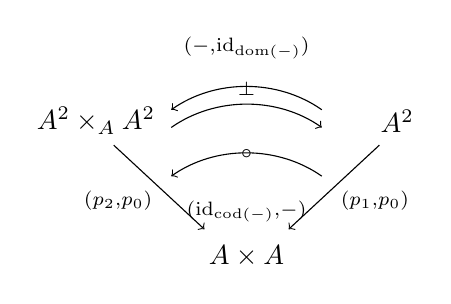
\begin{tikzpicture}[x=1.6em,y=1.6em]
  \node (x) at (-3.4,0.9) {$A^{2}\times_{A}A^{2}$};
  \node (y) at (3.4,0.9) {$A^{2}$};
  \draw[->] (1.7,1.15) .. controls (0.7,1.85) and (-0.7,1.85) .. (-1.7,1.15);
  \node at (0,2.55) {$\scriptstyle(-,\mathrm{id}_{\mathrm{dom}(-)})$};
  \node at (0,1.62) {$\scriptstyle\perp$};
  \draw[->] (-1.7,0.75) .. controls (-0.7,1.45) and (0.7,1.45) .. (1.7,0.75);
  \node at (0,0.15) {$\scriptstyle\circ$};
  \draw[->] (1.7,-0.35) .. controls (0.7,0.35) and (-0.7,0.35) .. (-1.7,-0.35);
  \node at (0,-1.15) {$\scriptstyle(\mathrm{id}_{\mathrm{cod}(-)},-)$};
  \draw[->] (-3.0,0.35) -- (-0.95,-1.55);
  \node at (-2.9,-0.9) {$\scriptstyle(p_{2},p_{0})$};
  \draw[->] (3.0,0.35) -- (0.95,-1.55);
  \node at (2.9,-0.9) {$\scriptstyle(p_{1},p_{0})$};
  \node (axa) at (0,-2.15) {$A\times A$};
\end{tikzpicture}
\end{center}

这个\trFiberedAdjunction{}使我们能够在∞-宇宙层面工作，而非纯粹在\trHomotopyTwoCategory{}中工作；它出现在 %
一条结果的证明中，该结果使我们能把\trLimit{}与\trColimit{}图表转换为右与左\trKanExtension{}图表 %
（见命题 4.3.4）。
\end{example}
\begin{proposition}\label{prop:absrl-cospan-hom}
下左所示\trCospan{}容许一个绝对右提升，当且仅当下右所示\trCospan{}容许一个绝对右提升
\begin{center}
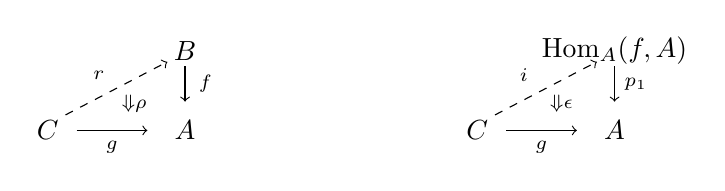
\begin{tikzpicture}[x=1.6em,y=1.6em]
  \node (b) at (2.2,1.5) {$B$};
  \draw[->] (2.2,1.15) -- (2.2,0.35);
  \node at (2.66,0.75) {$\scriptstyle f$};
  \node (d1) at (-0.9,-0.3) {$C$};
  \node (a1) at (2.2,-0.3) {$A$};
  \draw[->] (-0.25,-0.3) -- (1.35,-0.3);
  \node at (0.55,-0.68) {$\scriptstyle g$};
  \draw[->,dashed] (-0.5,0.05) -- (1.8,1.25);
  \node at (0.25,0.95) {$\scriptstyle r$};
  \node at (1.05,0.3) {$\scriptstyle\Downarrow\rho$};
  \begin{scope}[shift={(8.8,0)}]
  \node (h) at (3.1,1.5) {$\mathrm{Hom}_{A}(f,A)$};
  \draw[->] (3.1,1.15) -- (3.1,0.35);
  \node at (3.58,0.75) {$\scriptstyle p_{1}$};
  \node (d2) at (0,-0.3) {$C$};
  \node (a2) at (3.1,-0.3) {$A$};
  \draw[->] (0.65,-0.3) -- (2.25,-0.3);
  \node at (1.45,-0.68) {$\scriptstyle g$};
  \draw[->,dashed] (0.4,0.05) -- (2.7,1.25);
  \node at (1.05,0.95) {$\scriptstyle i$};
  \node at (1.9,0.3) {$\scriptstyle\Downarrow\epsilon$};
  \end{scope}
\end{tikzpicture}
\end{center}
此时 2-\trCell{} $\epsilon$ 必为\trIsomorphism，且对 $(i,\epsilon)$ 可取为 %
$(\qcor{\rho},\mathrm{id}_{g})$。
\end{proposition}

\begin{proof}
由定理 3.5.12 与\cref{cor:right-representability-terminal-element}，为验证存在性陈述，只需证明：%
$\mathrm{Hom}_{A}(f,g)$ 容许 $C$ 上的终元素，当且仅当 $\mathrm{Hom}_{A}(p_{1},g)$ 容许 $C$ 上的 %
终元素。

从构造\trCommaInfinityCategory{} $\mathrm{Hom}_{A}(p_{1},g)$ 的定义性\trPullback{} (3.4.2) 可见，%
$\mathrm{Hom}_{A}(p_{1},g)\cong\mathrm{Hom}_{A}(A,g)\times_{A}\mathrm{Hom}_{A}(f,A)$。
\begin{center}
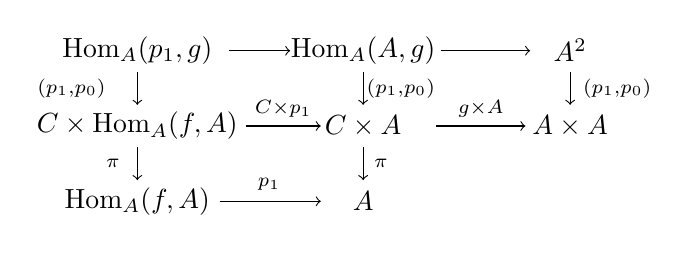
\begin{tikzpicture}[x=1.7em,y=1.7em]
  \node (t1) at (0,1.6) {$\mathrm{Hom}_{A}(p_{1},g)$};
  \node (t2) at (4.8,1.6) {$\mathrm{Hom}_{A}(A,g)$};
  \node (t3) at (9.2,1.6) {$A^{2}$};
  \node (m1) at (0,0) {$C\times\mathrm{Hom}_{A}(f,A)$};
  \node (m2) at (4.8,0) {$C\times A$};
  \node (m3) at (9.2,0) {$A\times A$};
  \node (b1) at (0,-1.6) {$\mathrm{Hom}_{A}(f,A)$};
  \node (b2) at (4.8,-1.6) {$A$};
  \draw[->] (1.95,1.6) -- (3.25,1.6);
  \draw[->] (6.45,1.6) -- (8.35,1.6);
  \draw[->] (2.3,0) -- (3.9,0);
  \node at (3.1,0.36) {$\scriptstyle C\times p_{1}$};
  \draw[->] (6.35,0) -- (8.25,0);
  \node at (7.3,0.36) {$\scriptstyle g\times A$};
  \draw[->] (1.75,-1.6) -- (3.9,-1.6);
  \node at (2.8,-1.24) {$\scriptstyle p_{1}$};
  \draw[->] (0,1.15) -- (0,0.45);
  \node at (-1.4,0.8) {$\scriptstyle(p_{1},p_{0})$};
  \draw[->] (4.8,1.15) -- (4.8,0.45);
  \node at (5.6,0.8) {$\scriptstyle(p_{1},p_{0})$};
  \draw[->] (9.2,1.15) -- (9.2,0.45);
  \node at (10.2,0.8) {$\scriptstyle(p_{1},p_{0})$};
  \draw[->] (0,-0.45) -- (0,-1.15);
  \node at (-0.52,-0.8) {$\scriptstyle\pi$};
  \draw[->] (4.8,-0.45) -- (4.8,-1.15);
  \node at (5.18,-0.8) {$\scriptstyle\pi$};
  \node at (0.52,1.12) {$\scriptstyle\lrcorner$};
  \node at (5.32,1.12) {$\scriptstyle\lrcorner$};
  \node at (0.52,-0.48) {$\scriptstyle\lrcorner$};
\end{tikzpicture}
\end{center}
于是，由\cref{lem:fibered-adjunction-pullback-projection}，\cref{exa:fibered-adjoints-composition} %
的「复合-恒同」\trFiberedAdjunction{}沿函子 $g\times f\colon C\times B\to A\times A$ 拉回，定义\trFiberedAdjunction
\begin{center}
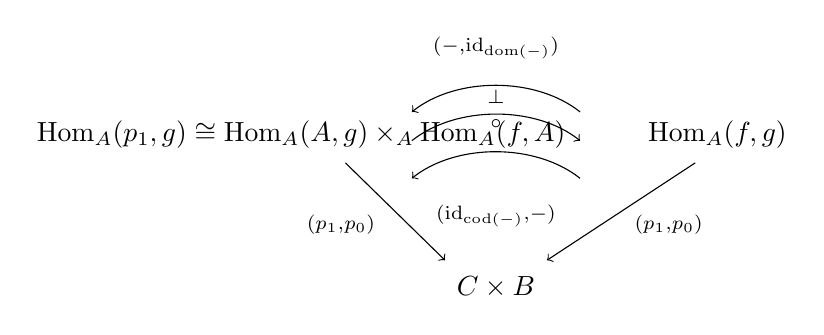
\begin{tikzpicture}[x=1.6em,y=1.6em]
  \node (x) at (-4.4,1.1) {$\mathrm{Hom}_{A}(p_{1},g)\cong\mathrm{Hom}_{A}(A,g)\times_{A}\mathrm{Hom}_{A}(f,A)$};
  \node (y) at (5.0,1.1) {$\mathrm{Hom}_{A}(f,g)$};
  \draw[->] (1.9,1.6) .. controls (0.9,2.4) and (-0.9,2.4) .. (-1.9,1.6);
  \node at (0,3.05) {$\scriptstyle(-,\mathrm{id}_{\mathrm{dom}(-)})$};
  \node at (0,1.95) {$\scriptstyle\perp$};
  \draw[->] (-1.9,0.95) .. controls (-0.9,1.75) and (0.9,1.75) .. (1.9,0.95);
  \node at (0,1.32) {$\scriptstyle\circ$};
  \draw[->] (1.9,0.1) .. controls (0.9,0.9) and (-0.9,0.9) .. (-1.9,0.1);
  \node at (0,-0.75) {$\scriptstyle(\mathrm{id}_{\mathrm{cod}(-)},-)$};
  \draw[->] (-3.4,0.45) -- (-1.15,-1.75);
  \node at (-3.5,-0.95) {$\scriptstyle(p_{1},p_{0})$};
  \draw[->] (4.5,0.45) -- (1.15,-1.75);
  \node at (3.9,-0.95) {$\scriptstyle(p_{1},p_{0})$};
  \node (cb) at (0,-2.35) {$C\times B$};
\end{tikzpicture}
\end{center}
后者再与投影 $\pi\colon C\times B\twoheadrightarrow C$ 复合，给出 $C$ 之上的\trFiberedAdjunction
\begin{center}
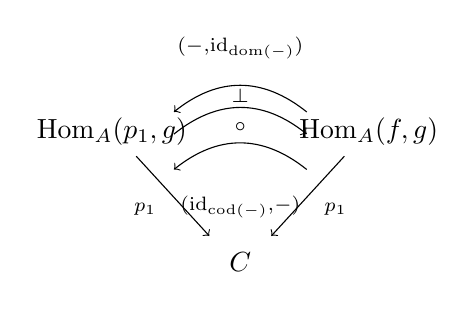
\begin{tikzpicture}[x=1.6em,y=1.6em]
  \node (x) at (-2.9,0.9) {$\mathrm{Hom}_{A}(p_{1},g)$};
  \node (y) at (2.9,0.9) {$\mathrm{Hom}_{A}(f,g)$};
  \draw[->] (1.5,1.35) .. controls (0.5,2.15) and (-0.5,2.15) .. (-1.5,1.35);
  \node at (0,2.8) {$\scriptstyle(-,\mathrm{id}_{\mathrm{dom}(-)})$};
  \node at (0,1.72) {$\scriptstyle\perp$};
  \draw[->] (-1.5,0.85) .. controls (-0.5,1.65) and (0.5,1.65) .. (1.5,0.85);
  \node at (0,1.02) {$\scriptstyle\circ$};
  \draw[->] (1.5,0.05) .. controls (0.5,0.85) and (-0.5,0.85) .. (-1.5,0.05);
  \node at (0,-0.8) {$\scriptstyle(\mathrm{id}_{\mathrm{cod}(-)},-)$};
  \draw[->] (-2.35,0.35) -- (-0.7,-1.45);
  \node at (-2.15,-0.85) {$\scriptstyle p_{1}$};
  \draw[->] (2.35,0.35) -- (0.7,-1.45);
  \node at (2.15,-0.85) {$\scriptstyle p_{1}$};
  \node (c) at (0,-2.05) {$C$};
\end{tikzpicture}
\end{center}
它介于 $\mathrm{Hom}_{A}(p_{1},g)$ 的余定义域投影与 $\mathrm{Hom}_{A}(f,g)$ 的余定义域投影之间——%
二者视为 $C$ 之上的切片\trInfinityCosmos{}的对象。由于我们有两个方向的\trRightAdjoint，据定理 2.4.2，%
任何一侧上的终元素都被相应的\trRightAdjoint{}带到另一侧上的终元素。这证明了诸绝对右提升条件的 %
等价性。

现在我们假定两个绝对右提升中有一个从而两者都存在。注意最右的伴随 %
$(\mathrm{id}_{\mathrm{cod}(-)},-)\colon\mathrm{Hom}_{A}(f,g)\to\mathrm{Hom}_{A}(p_{1},g)$ 由粘贴等式
\begin{center}
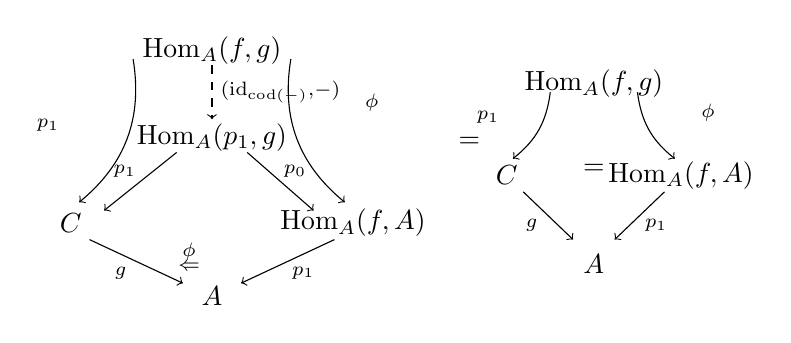
\begin{tikzpicture}[x=1.5em,y=1.5em]
  \node (homfg) at (0,3.4) {$\mathrm{Hom}_{A}(f,g)$};
  \node (hompg) at (0,1.3) {$\mathrm{Hom}_{A}(p_{1},g)$};
  \draw[->,dashed] (0,3.05) -- (0,1.75);
  \node at (1.65,2.4) {$\scriptstyle(\mathrm{id}_{\mathrm{cod}(-)},-)$};
  \draw[->] (-1.9,3.2) to[bend left=30] (-3.2,-0.25);
  \node at (-3.95,1.6) {$\scriptstyle p_{1}$};
  \draw[->] (1.9,3.2) to[bend right=30] (3.2,-0.25);
  \node at (3.85,2.15) {$\scriptstyle\qcor{\phi}$};
  \node (c) at (-3.4,-0.75) {$C$};
  \node (homfa) at (3.4,-0.75) {$\mathrm{Hom}_{A}(f,A)$};
  \draw[->] (-0.85,0.95) -- (-2.6,-0.45);
  \node at (-2.1,0.5) {$\scriptstyle p_{1}$};
  \draw[->] (0.85,0.95) -- (2.45,-0.45);
  \node at (2.0,0.5) {$\scriptstyle p_{0}$};
  \node (a) at (0,-2.5) {$A$};
  \draw[->] (-2.95,-1.15) -- (-0.7,-2.2);
  \node at (-2.2,-1.95) {$\scriptstyle g$};
  \draw[->] (2.95,-1.15) -- (0.7,-2.2);
  \node at (2.2,-1.95) {$\scriptstyle p_{1}$};
  \node at (-0.55,-1.45) {$\scriptstyle\phi$};
  \node at (-0.55,-1.8) {$\scriptstyle\Leftarrow$};
  \node at (6.2,1.2) {$=$};
  \begin{scope}[shift={(9.2,0)}]
  \node (homfg2) at (0,2.6) {$\mathrm{Hom}_{A}(f,g)$};
  \node (c2) at (-2.1,0.4) {$C$};
  \node (homfa2) at (2.1,0.4) {$\mathrm{Hom}_{A}(f,A)$};
  \draw[->] (-1.05,2.4) to[bend left=22] (-1.95,0.8);
  \node at (-2.55,1.8) {$\scriptstyle p_{1}$};
  \draw[->] (1.05,2.4) to[bend right=22] (1.95,0.8);
  \node at (2.75,1.9) {$\scriptstyle\qcor{\phi}$};
  \node at (0,0.55) {$=$};
  \draw[->] (-1.7,0.0) -- (-0.5,-1.15);
  \node at (-1.5,-0.8) {$\scriptstyle g$};
  \draw[->] (1.7,0.0) -- (0.5,-1.15);
  \node at (1.5,-0.8) {$\scriptstyle p_{1}$};
  \node (a2) at (0,-1.75) {$A$};
  \end{scope}
\end{tikzpicture}
\end{center}
其中 $\qcor{\phi}\colon\mathrm{Hom}_{A}(f,g)\to\mathrm{Hom}_{A}(f,A)$ 是编码如下因子分解的%
\trFunctor：把 $\mathrm{Hom}_{A}(f,g)$ 的\trCommaCone{}穿过 $\mathrm{Hom}_{A}(f,A)$ 的%
\trCommaCone{}作因子分解。由定理 3.5.12，函子 $\qcor{\rho}\colon C\to\mathrm{Hom}_{A}(f,g)$ 定义 %
$p_{1}\colon\mathrm{Hom}_{A}(f,g)\twoheadrightarrow C$ 的一个\trRightAdjoint\trRightInverse。于是，%
据刚才的论证，$\qcor{\rho}$ 与 $(\mathrm{id}_{\mathrm{cod}(-)},-)$ 的复合定义 %
$p_{1}\colon\mathrm{Hom}_{A}(p_{1},g)\twoheadrightarrow C$ 的一个\trRightAdjoint\trRightInverse，%
编码 $g$ 穿过 $p_{1}$ 的绝对右提升之数据，且必然\trIsomorphism{}于对 $(i,\epsilon)$。粘贴等式
\begin{center}
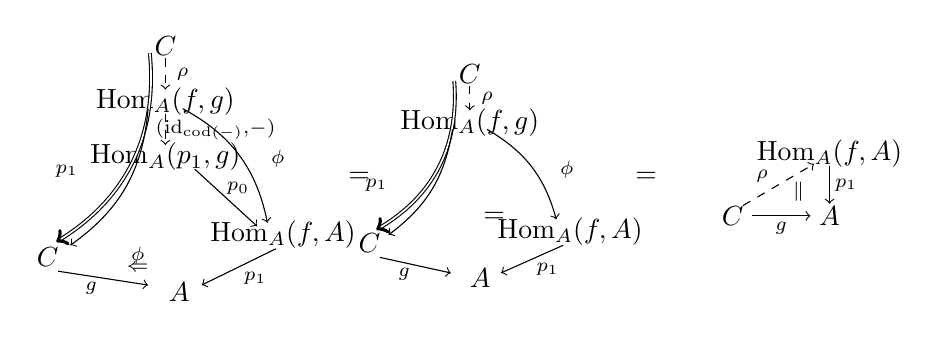
\begin{tikzpicture}[x=1.25em,y=1.25em]
  \node (ctop) at (0,4.6) {$C$};
  \draw[->,dashed] (0,4.25) -- (0,3.35);
  \node at (0.5,3.8) {$\scriptstyle\qcor{\rho}$};
  \node (homfg) at (0,3.0) {$\mathrm{Hom}_{A}(f,g)$};
  \draw[->,dashed] (0,2.65) -- (0,1.75);
  \node at (1.45,2.2) {$\scriptstyle(\mathrm{id}_{\mathrm{cod}(-)},-)$};
  \node (hompg) at (0,1.4) {$\mathrm{Hom}_{A}(p_{1},g)$};
  \node (cb) at (-3.4,-1.5) {$C$};
  \draw[double,->] (-0.45,4.4) to[bend left=32] (-3.15,-1.05);
  \draw[->] (-0.5,2.8) to[bend left=25] (-2.75,-1.15);
  \node at (-2.85,1.0) {$\scriptstyle p_{1}$};
  \node (homfa) at (3.4,-0.85) {$\mathrm{Hom}_{A}(f,A)$};
  \draw[->] (0.5,2.8) to[bend left=25] (2.95,-0.5);
  \node at (3.25,1.35) {$\scriptstyle\qcor{\phi}$};
  \draw[->] (0.85,1.05) -- (2.65,-0.6);
  \node at (2.1,0.5) {$\scriptstyle p_{0}$};
  \node (a) at (0.4,-2.5) {$A$};
  \draw[->] (-3.1,-1.9) -- (-0.5,-2.3);
  \node at (-2.15,-2.4) {$\scriptstyle g$};
  \draw[->] (3.2,-1.25) -- (1.05,-2.3);
  \node at (2.6,-2.1) {$\scriptstyle p_{1}$};
  \node at (-0.8,-1.45) {$\scriptstyle\phi$};
  \node at (-0.8,-1.8) {$\scriptstyle\Leftarrow$};
  \node at (5.6,0.8) {$=$};
  \begin{scope}[shift={(8.8,0)}]
  \node (c2top) at (0,3.8) {$C$};
  \draw[->,dashed] (0,3.45) -- (0,2.75);
  \node at (0.5,3.1) {$\scriptstyle\qcor{\rho}$};
  \node (homfg2) at (0,2.4) {$\mathrm{Hom}_{A}(f,g)$};
  \node (c2b) at (-2.9,-1.1) {$C$};
  \draw[double,->] (-0.45,3.6) to[bend left=32] (-2.7,-0.7);
  \draw[->] (-0.5,2.2) to[bend left=22] (-2.35,-0.85);
  \node at (-2.7,0.6) {$\scriptstyle p_{1}$};
  \node (homfa2) at (2.9,-0.75) {$\mathrm{Hom}_{A}(f,A)$};
  \draw[->] (0.5,2.2) to[bend left=22] (2.5,-0.4);
  \node at (2.8,1.05) {$\scriptstyle\qcor{\phi}$};
  \node at (0.7,-0.35) {$=$};
  \node (a2) at (0.3,-2.1) {$A$};
  \draw[->] (-2.6,-1.5) -- (-0.55,-1.95);
  \node at (-1.9,-2.0) {$\scriptstyle g$};
  \draw[->] (2.7,-1.15) -- (0.9,-1.95);
  \node at (2.25,-1.85) {$\scriptstyle p_{1}$};
  \end{scope}
  \node at (13.9,0.8) {$=$};
  \begin{scope}[shift={(16.4,0)}]
  \node (c3) at (0,-0.3) {$C$};
  \node (a3) at (2.8,-0.3) {$A$};
  \draw[->] (0.55,-0.3) -- (2.25,-0.3);
  \node at (1.4,-0.66) {$\scriptstyle g$};
  \node (homfa3) at (2.8,1.5) {$\mathrm{Hom}_{A}(f,A)$};
  \draw[->,dashed] (0.3,0.0) -- (2.35,1.2);
  \node at (0.85,0.85) {$\scriptstyle\qcor{\rho}$};
  \node at (1.9,0.4) {$\scriptstyle\parallel$};
  \draw[->] (2.8,1.15) -- (2.8,0.05);
  \node at (3.28,0.6) {$\scriptstyle p_{1}$};
  \end{scope}
\end{tikzpicture}
\end{center}
表明这个绝对右提升图表由 $(\qcor{\rho},\mathrm{id}_{g})$ 给出，如所宣称。
\end{proof}

下面的例子暗示\cref{prop:absrl-cospan-hom}的一个应用。

\begin{example}\label{exa:left-representation-cone}
由与单纯集的映射 $f\colon U\to V$ 作余张量所诱导的\trFunctor{} $A^{f}\colon A^{V}\to A^{U}$ 的 %
左表示，本身可定义为与一个单纯集的余张量，该单纯集由通过映射 $f$ 把 $V$ 贴到 %
\textbf{柱}（cylinder）$U\times\qcTwo$ 的定义域端而形成：
\begin{center}
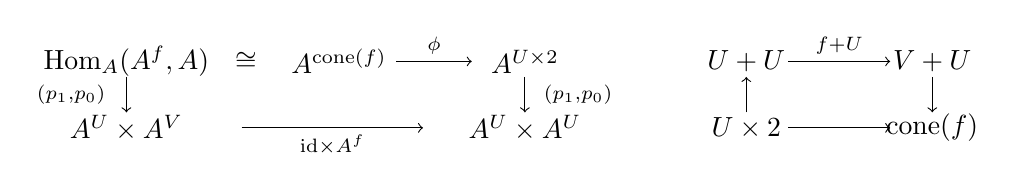
\begin{tikzpicture}[x=1.6em,y=1.6em]
  \node (tl) at (0,1.5) {$\mathrm{Hom}_{A}(A^{f},A)$};
  \node (eq) at (2.7,1.5) {$\cong$};
  \node (tc) at (4.8,1.5) {$A^{\mathrm{cone}(f)}$};
  \node (tr) at (9.0,1.5) {$A^{U\times 2}$};
  \draw[->] (6.1,1.5) -- (7.8,1.5);
  \node at (6.95,1.86) {$\scriptstyle\qcor{\phi}$};
  \node at (3.72,1.02) {$\scriptstyle\lrcorner$};
  \draw[->] (0,1.15) -- (0,0.35);
  \node at (-1.25,0.75) {$\scriptstyle(p_{1},p_{0})$};
  \draw[->] (9.0,1.15) -- (9.0,0.35);
  \node at (10.2,0.75) {$\scriptstyle(p_{1},p_{0})$};
  \node (bl) at (0,0) {$A^{U}\times A^{V}$};
  \node (br) at (9.0,0) {$A^{U}\times A^{U}$};
  \draw[->] (2.6,0) -- (6.7,0);
  \node at (4.65,-0.38) {$\scriptstyle\mathrm{id}\times A^{f}$};
  \begin{scope}[shift={(14.0,0)}]
  \node (ul) at (0,1.5) {$U+U$};
  \node (ur) at (4.2,1.5) {$V+U$};
  \draw[->] (0.95,1.5) -- (3.25,1.5);
  \node at (2.1,1.86) {$\scriptstyle f+U$};
  \draw[->] (0,0.35) -- (0,1.15);
  \draw[->] (4.2,1.15) -- (4.2,0.35);
  \node (ll) at (0,0) {$U\times 2$};
  \node (lr) at (4.2,0) {$\mathrm{cone}(f)$};
  \draw[->] (0.95,0) -- (3.25,0);
  \node at (0.52,0.42) {$\scriptstyle\lrcorner$};
  \end{scope}
\end{tikzpicture}
\end{center}
\cref{prop:absrl-cospan-hom}在绝对右提升问题
\begin{center}
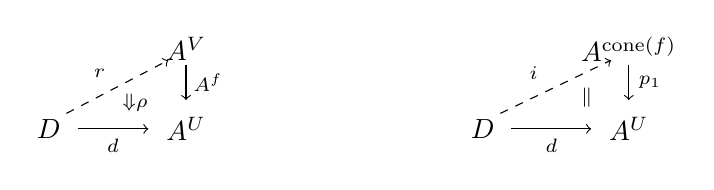
\begin{tikzpicture}[x=1.6em,y=1.6em]
  \node (av) at (2.2,1.5) {$A^{V}$};
  \draw[->] (2.2,1.15) -- (2.2,0.35);
  \node at (2.7,0.75) {$\scriptstyle A^{f}$};
  \node (d1) at (-0.9,-0.3) {$D$};
  \node (au) at (2.2,-0.3) {$A^{U}$};
  \draw[->] (-0.25,-0.3) -- (1.35,-0.3);
  \node at (0.55,-0.68) {$\scriptstyle d$};
  \draw[->,dashed] (-0.5,0.05) -- (1.8,1.25);
  \node at (0.25,0.95) {$\scriptstyle r$};
  \node at (1.05,0.3) {$\scriptstyle\Downarrow\rho$};
  \begin{scope}[shift={(9.4,0)}]
  \node (acf) at (2.8,1.5) {$A^{\mathrm{cone}(f)}$};
  \draw[->] (2.8,1.15) -- (2.8,0.35);
  \node at (3.28,0.75) {$\scriptstyle p_{1}$};
  \node (d2) at (-0.5,-0.3) {$D$};
  \node (au2) at (2.8,-0.3) {$A^{U}$};
  \draw[->] (0.15,-0.3) -- (1.95,-0.3);
  \node at (1.05,-0.68) {$\scriptstyle d$};
  \draw[->,dashed] (-0.1,0.05) -- (2.4,1.25);
  \node at (0.65,0.95) {$\scriptstyle i$};
  \node at (1.85,0.4) {$\scriptstyle\parallel$};
  \end{scope}
\end{tikzpicture}
\end{center}
之间建立一个对应；在此对应下，单一\trFunctor{} $i\colon D\to A^{\mathrm{cone}(f)}$ 同时用来编码 %
\trFunctor
\[
r:=D\xrightarrow{\;i\;}A^{\mathrm{cone}(f)}\xrightarrow{\;p_{0}\;}A^{V}
\]
与\trNaturalTransformation
\[
\qcor{\rho}:=D\xrightarrow{\;i\;}A^{\mathrm{cone}(f)}\xrightarrow{\;\qcor{\phi}\;}A^{U\times 2}
\]
的数据。
\end{example}

\subsection*{练习}

\begin{exercise}\label{ex:ambient-equivalence}
设 $B$ 是一个 2-范畴中的对象，并考虑 $B$ 上的诸\trIsofibration{}之间的一个映射
\begin{center}
\begin{tikzpicture}[x=1.5em,y=1.5em]
  \node (e) at (-1.9,1.3) {$E$};
  \node (f) at (1.9,1.3) {$F$};
  \draw[->] (-1.15,1.3) -- (1.15,1.3);
  \node at (0,1.7) {$\scriptstyle f$};
  \draw[->] (-1.5,0.85) -- (-0.45,-0.95);
  \draw[->] (1.5,0.85) -- (0.45,-0.95);
  \node (b) at (0,-1.5) {$B$};
\end{tikzpicture}
\end{center}
证明：若 $f$ 在所在的 2-范畴中是一个\trEquivalence，则 $f$ 在「$B$ 之上的等价纤维化之切片 %
2-范畴」——其 1-\trCell{}构成 $B$ 上的交换三角形，其 2-\trCell{}按「与余定义域\trIsofibration{}作%
\trWhiskering{}后给出定义域\trIsofibration{}上的恒同 2-\trCell」之意义居于 $B$ 之上——中也是 %
一个\trEquivalence。
\end{exercise}

\begin{exercise}\label{ex:cheap-yoneda-fibered-equivalence}
在推论 3.5.11 的对应之下，证明下列诸条等价：
\begin{enumerate}[label=(\roman*)]
\item $\alpha\colon f\Rightarrow g$ 是一个\trIsomorphism；
\item 函子 $\qcor{\alpha_{*}}\colon\mathrm{Hom}_{B}(B,f)\to\mathrm{Hom}_{B}(B,g)$ 定义 %
$A\times B$ 之上的一个\trFiberedEquivalence；
\item 函子 $\qcor{\alpha^{*}}\colon\mathrm{Hom}_{B}(g,B)\to\mathrm{Hom}_{B}(f,B)$ 定义 %
$B\times A$ 之上的一个\trFiberedEquivalence。
\end{enumerate}
\end{exercise}

\begin{exercise}\label{ex:smothering-lifts-adjunctions}
设 $F\colon\mathcal{A}\to\mathcal{B}$ 是一个覆盖 2-函子。用引理 2.1.11 证明：$\mathcal{B}$ 中的 %
任何\trAdjunction{}都可以提升为 $\mathcal{A}$ 中的\trAdjunction。进而证明：若我们先已指定了对象与 %
1-\trCell{}的提升、以及 $\mathcal{B}$ 中\trAdjunction{}的\trUnit{}或\trCounit{}之一，则存在余下那个 %
2-\trCell{}的提升，它与先已指定的数据组合起来定义 $\mathcal{A}$ 中的一个\trAdjunction。这证明了 %
\cref{lem:smothering-lift-adjunctions}的一个更精确的版本。
\end{exercise}

\begin{exercise}\label{ex:square-preserves-absrl}
扩展\cref{prop:absrl-cospan-hom}的证明以证明：一个方块保持绝对右提升 $(r,\rho)$，当且仅当诱导方块 %
保持绝对右提升 $(i,\epsilon)$：
\begin{center}
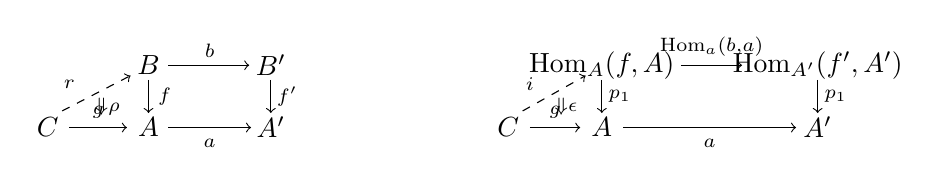
\begin{tikzpicture}[x=1.3em,y=1.5em]
  \node (b) at (0,1.5) {$B$};
  \node (bp) at (3.4,1.5) {$B'$};
  \draw[->] (0.55,1.5) -- (2.8,1.5);
  \node at (1.7,1.86) {$\scriptstyle b$};
  \draw[->] (0,1.15) -- (0,0.35);
  \node at (0.45,0.75) {$\scriptstyle f$};
  \draw[->] (3.4,1.15) -- (3.4,0.35);
  \node at (3.85,0.75) {$\scriptstyle f'$};
  \node (c) at (-2.8,0) {$C$};
  \node (a) at (0,0) {$A$};
  \node (ap) at (3.4,0) {$A'$};
  \draw[->] (-2.2,0) -- (-0.6,0);
  \node at (-1.4,0.36) {$\scriptstyle g$};
  \draw[->] (0.55,0) -- (2.85,0);
  \node at (1.7,-0.38) {$\scriptstyle a$};
  \draw[->,dashed] (-2.4,0.4) -- (-0.5,1.25);
  \node at (-2.2,1.05) {$\scriptstyle r$};
  \node at (-1.15,0.5) {$\scriptstyle\Downarrow\rho$};
  \begin{scope}[shift={(12.6,0)}]
  \node (h1) at (0,1.5) {$\mathrm{Hom}_{A}(f,A)$};
  \node (h2) at (6.0,1.5) {$\mathrm{Hom}_{A'}(f',A')$};
  \draw[->] (2.2,1.5) -- (3.9,1.5);
  \node at (3.05,1.95) {$\scriptstyle\mathrm{Hom}_{a}(b,a)$};
  \draw[->] (0,1.15) -- (0,0.35);
  \node at (0.5,0.75) {$\scriptstyle p_{1}$};
  \draw[->] (6.0,1.15) -- (6.0,0.35);
  \node at (6.5,0.75) {$\scriptstyle p_{1}$};
  \node (c2) at (-2.6,0) {$C$};
  \node (a2) at (0,0) {$A$};
  \node (a3) at (6.0,0) {$A'$};
  \draw[->] (-2.0,0) -- (-0.6,0);
  \node at (-1.3,0.36) {$\scriptstyle g$};
  \draw[->] (0.6,0) -- (5.4,0);
  \node at (3.0,-0.38) {$\scriptstyle a$};
  \draw[->,dashed] (-2.2,0.4) -- (-0.45,1.25);
  \node at (-2.0,1.05) {$\scriptstyle i$};
  \node at (-1.0,0.5) {$\scriptstyle\Downarrow\epsilon$};
  \end{scope}
\end{tikzpicture}
\end{center}
\end{exercise}
